\documentclass[titlepage]{article}

\usepackage{amsmath}
\usepackage{amssymb}
\usepackage{fullpage}
\usepackage{graphicx}

\DeclareMathOperator{\arccot}{arccot}

\title{Assignment 2}
\date{\today}
\author{Jerry Jiang\\ TianQi Shi}

\begin{document}
\maketitle

\noindent
\section{Problem Set 1}
\subsection{Problem 1}
a) $y' + 3x^2y^2 = 0, y(0) = 1$
\begin{align*}
  & y' + 3x^2y^2 = 0, y(0) = 1
  \\ & y' = -3x^2y^2
  \\ & \frac{dy}{dx} = -3x^2y^2
  \\ & \frac{dy}{y^2} = -3x^2 dx
  \\ \int & \frac{dy}{y^2} = \int -3x^2 dx
  \\ & \frac{-1}{y} = -x^3 + C
  \\ & -1 = (-x^3 + C)y
  \\ & y = \frac{-1}{-x^3 + C}
\end{align*}

Particular solution:

\begin{align*}
  & y = \frac{-1}{-x^3 + C}
  \\ & 1 = \frac{-1}{0 + C}
  \\ & 1 = \frac{-1}{C}
  \\ & C = -1
\end{align*}

$$\therefore y = \frac{-1}{-x^3 - 1} = \frac{1}{x^3 + 1}$$


\noindent
b) $x^2y' = 1 + y^2$

\begin{align*}
  & x^2y' = 1 + y^2
  \\ & \frac{dyx^2}{dx} = 1 + y^2
  \\ & \frac{dy}{1 + y^2} = \frac{1}{x^2} dx
  \\ \int & \frac{dy}{1 + y^2} = \int \frac{1}{x^2} dx
  \\ & \arctan y = \frac{-1}{x} + C
  \\ & y = \tan(\frac{-1}{x} + C) \end{align*}

\subsection{Problem 2}

\begin{align*}
  & (x-1)y' + \frac{2(x-1)y}{x} = (x-1)(x+1)
  \\ & y' + \frac{2y}{x} = x+1 \tag{$x \neq 1$}
  \\ & \sigma y' + \sigma \frac{2y}{x} = \sigma(x+1)
\end{align*}

Use integrating factor method:

\begin{align*}
  & (\sigma y)' = \sigma y' + \sigma' y = \sigma y' + \sigma \frac{2y}{x}
  \\ & \sigma' y = \sigma \frac{2y}{x}
  \\ & \sigma' = \sigma \frac{2}{x}
  \\ & \frac{d\sigma}{dx} = \sigma \frac{2}{x}
  \\ & \frac{d\sigma}{\sigma} = \frac{2}{x} dx
  \\ \int & \frac{d\sigma}{\sigma} = \int \frac{2}{x} dx
  \\ & \ln|\sigma| = 2 \ln|x| + C
  \\ & |\sigma| = e^C|x|^2 \tag{$x \neq 0$}
  \\ & \sigma = Dx^2
\end{align*}

Calculate $y$:

\begin{align*}
  & \frac{dDx^2y}{dx} = Dx^2(x+1)
  \\ & \frac{dx^2y}{dx} = x^2(x+1)
  \\ & dx^2y = x^2(x+1) dx
  \\ & dx^2y = x^3 + x^2 dx
  \\ \int & dx^2y = \int x^3 + x^2 dx
  \\ & x^2y = \frac{x^4}{4} + \frac{x^3}{3} + C
  \\ & y = \frac{x^2}{4} + \frac{x}{3} + \frac{C}{x^2} \tag{$x \neq 0 $}
\end{align*}

In addition, $x \neq 1$, since we divided the original equation by $(x-1)$.

Find particular solution:

\begin{align*}
  & y = \frac{x^2}{4} + \frac{x}{3} + \frac{C}{x^2}
  \\ & \frac{7}{3} = \frac{2^2}{4} + \frac{2}{3} + \frac{C}{2^2}
  \\ & \frac{7}{3} = 1 + \frac{2}{3} + \frac{C}{4}
  \\ & \frac{7}{3} = \frac{5}{3} + \frac{C}{4}
  \\ & \frac{2}{3} = \frac{C}{4}
  \\ & \frac{8}{3} = C
\end{align*}

$$\therefore y = \frac{x^2}{4} + \frac{x}{3} + \frac{8}{3x^2}$$

\section{Problem Set 2}
\subsection{Problem 1}
Given the linear equation $xy' - y = x - 1$, solve for $y(x)$.
\\ a) $y(e) = 1$
\\ \\ Using the integrating factor method, first multiply all terms by the integrating factor $\sigma$:
\begin{align*}
xy' - y &= x - 1
\\ y' - \frac{y}{x} &= 1 - \frac{1}{x}
\\ \sigma y' - \sigma \frac{y}{x} &= \sigma - \sigma \frac{1}{x}
\end{align*}
Set the left hand side to $(\sigma y)'$:
\begin{align*}
(\sigma y)' &= \sigma y' - \sigma \frac{y}{x}
\\ \sigma y' + \sigma'y &= \sigma y' - \sigma \frac{y}{x}
\\ \sigma'y &= - \sigma \frac{y}{x}
\\ \frac{d\sigma}{dx} &= - \frac{\sigma}{x}
\\ \frac{d\sigma}{\sigma} &= - \frac{dx}{x}
\\ \ln \left| \sigma \right| &= - \ln \left| x \right|
\\ \sigma &= \frac{1}{x}
\end{align*}
Then set the right hand side to $\frac{d}{dx} (\sigma y)$:
\begin{align*}
\frac{d}{dx} (\frac{y}{x}) &= \frac{1}{x} - \frac{1}{x}\frac{1}{x}
\\ \int d (\frac{y}{x}) &= \int \frac{1}{x} - \frac{1}{x^2} dx
\\ \frac{y}{x} &= \ln \left| x \right| + \frac{1}{x} + c
\\ y &= x\ln \left| x \right| + cx + 1
\end{align*}
Substituting initial conditions,
\begin{align*}
1 &= e\ln \left| e \right| + ce + 1
\\ 0 &= (c + 1)e
\\ c &= - 1
\end{align*}
$$ \therefore y = x\ln \left| x \right| - x + 1 $$

\noindent
b) $y (-1) = 1$
\\ Using the same general solution, substitute initial conditions.
\begin{align*}
1 &= (-1)\ln \left| (-1) \right| + c(-1) + 1
\\ c &= 0
\end{align*}
$$ \therefore y = x\ln \left| x \right| + 1 $$

\noindent
c) $y (0) = 1$
\\ The general solution contains a term $\ln \left| x \right|$ and the natural logarithm is indeterminate at $x=0$. Therefore, there is no particular solution satisfying this initial condition.


\subsection{Problem 2}
Solve for $y(x)$ given initial condition y(0) = -2:
\begin{align*}
y' &= \frac{e^x}{2y}
\\ \frac{dy}{dx} &= \frac{e^x}{2y}
\\ \int 2y dy &= \int e^x dx
\\ y^2 &= e^x + c
\\ y &= e^{\frac{x}{2}} + c
\end{align*}
Substituting initial conditions,
\begin{align*}
-2 &= e^{\frac{0}{2}} + c
\\ c &= -2
\end{align*}
Thus $y(x) = e^{\frac{x}{2}} - 2$

\subsection{Simulation}
To get the state space for the simulation, we start by defining two linear differential equations.
$$y_1(t) = x(t)$$
$$y_2(t) = x'(t)$$
If we differentiate both sides,
$$y_1'(t) = x'(t) = y_2(t)$$
$$y_2'(t) = -\frac{c}{m} x' - \frac{k}{m}x$$
We substitute these into the state space vector. Below is the MATLAB code used in the simulation:
\begin{verbatim}
% MSDamper.m
function dx = MSDamper(t,x,m,k,c)
%This program generates the Mass Spring Damper system equation mx''+cx'+ kx = 0.
% where m is the mass of the system
% k is the stiffness of the spring
% c is the viscosity damping
% x is displacement.

xd1 = x(2); %%first order derivative
xd2 = -(c/m)*x(2) - (k/m)*x(1);  %%second order derivative

dx = [xd1; xd2];
end


% solver.m
clc; clear all; close all;
% Solve the MSDamper function under different conditions

%initial conditions
m =  1;     %mass of the system
k =  1;     % stiffness of the spring
c =  1;     %viscosity damping
t_max = 5;  %simulation time 5 s

%options = odeset('Refine',6,'RelTol',1e-4);
x_0 =  0;   %initial displacement
x_d_0 = 1; %initial velocity
X_0 = [x_0; x_d_0];  %initial condition

[t,y] = ode45(@MSDamper, [0,t_max], X_0,[],m,k,c);
%y(:,1) is the Displacement; y(:,2) is the velocity

subplot(2,1,1),plot(t,y(:,1));
xlabel('Time (sec.)');
ylabel('Displacement (m)');
title('Mass-Spring systems');
subplot(2,1,2),plot(t,y(:,2));
xlabel('Time (sec.)');
ylabel('Velocity (m/sec.)');
\end{verbatim}

\noindent Using the initial values in the code here, we can produce the following.

\begin{center}
        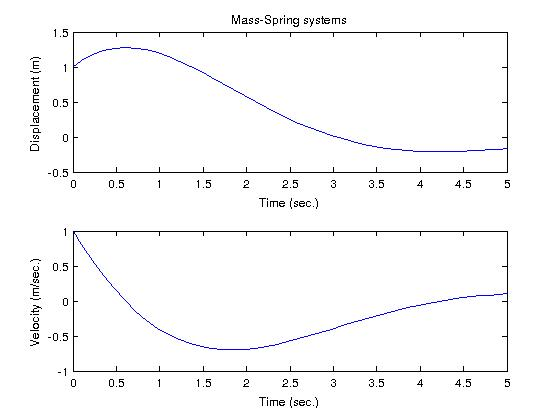
\includegraphics[scale=0.6]{matlab/base.jpg}
\end{center}

\noindent From these two charts, we can see that the spring oscillates in its displacement. The spring constant is small so oscillation occurs slowly, showing less than one full phase in the diagram. If we increase the spring constant $k$, we get a stiffer spring that oscillates more frequently in the same time frame. Also note that the following spring system has initial displacement 200 m and initial velocity 0 m/sec.

\begin{center}
        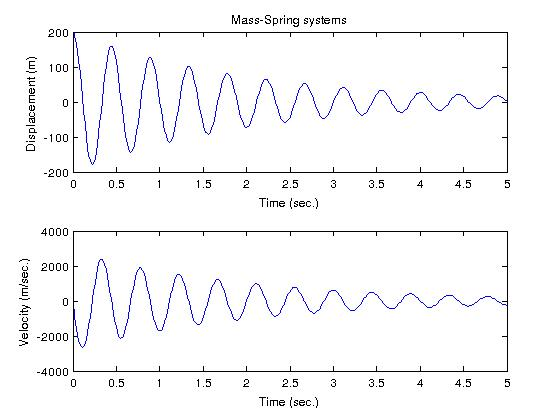
\includegraphics[scale=0.6]{matlab/k200.jpg}
\end{center}

\noindent Analyzing the viscocity damping coefficient $c$, we find that when $c > 0$ (as in the initial conditions) the oscillations are damped and amplitudes eventually go to 0. When $c = 0$, the oscillations are not damped and amplitude is always the same.

\begin{center}
        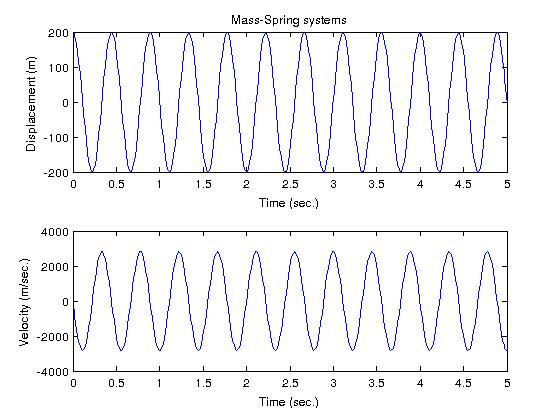
\includegraphics[scale=0.6]{matlab/d200k200c0.jpg}
\end{center}

\noindent When $c < 0$, the oscillations are damped negatively so they actually grow in size. The original amplitude is near 0 as we start with 0 initial displacement and velocity. However, the end behaviour has much higher amplitudes.

\begin{center}
        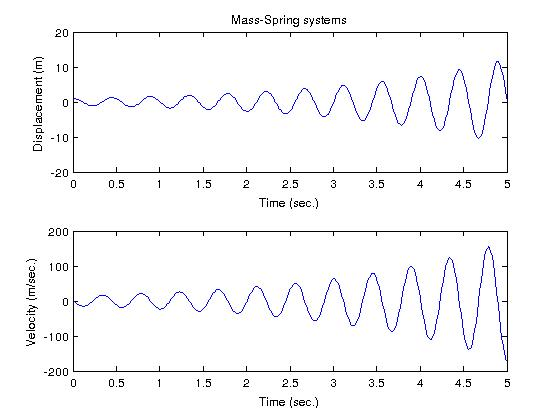
\includegraphics[scale=0.6]{matlab/k200c-1.jpg}
\end{center}

\end{document}
